\documentclass[11pt,twoside,a4paper]{book}  
% definice dokumentu
\usepackage[english]{babel}
\usepackage[T1]{fontenc} 				% pouzije EC fonty 
\usepackage[utf8]{inputenc} 			% utf8 kódování vstupu 
\usepackage[square, numbers]{natbib}	% sazba pouzite literatury
%\usepackage{indentfirst} 				% 1. odstavec jako v cestine, pro práci v aj možno zakomentovat
\usepackage{fancyhdr}					% tisk hlaviček a patiček stránek
\usepackage{nomencl} 					% umožňuje snadno definovat zkratky a jejich seznam

%%%%%%%%%%%%%%%%%%%%%%%%%%%%%%%%%%%%%%%%%%%%%%%%%%%%%%%%%%%%%%%
% informace o práci
\newcommand\WorkTitle{Interactive Visualization System for Hybrid Active Pixel Detectors Within the ATLAS Experiment at CERN}		% název
\newcommand\FirstandFamilyName{Petr Mánek}																							% autor
\newcommand\Supervisor{Ing. Stanislav Pospíšil, DrSc.}																				% vedoucí

\newcommand\TypeOfWork{Bachelor's Project}	% typ práce [Diplomová práce | Bakalářská práce | Bachelor's Project | Master's Thesis ]	

% Nastavte následují podle vašeho oboru a programu (pomoc hledejte na http://www.fel.cvut.cz/cz/education/bk/prehled.html)								
\newcommand\StudProgram{Open Informatics}											% program
\newcommand\StudBranch{Computer and Information Science}           					% obor

%%%%%%%%%%%%%%%%%%%%%%%%%%%%%%%%%%%%%%%%%%%%%%%%%%%%%%%%%%%%%%%
% minimální importy
\usepackage{graphicx}					% pro vkládání obrázků
\usepackage{k336_thesis_macros} 		% specialni makra pro formatovani DP a BP
\usepackage[
pdftitle={\WorkTitle},				% nastaví v informacích o pdf název
pdfauthor={\FirstandFamilyName},	% nastaví v informacích o pdf autora
colorlinks=true,					% před tiskem doporučujeme nastavit na false, aby odkazy a url nebyly šedé při ČB tisku
breaklinks=true,
urlcolor=red,
citecolor=blue,
linkcolor=blue,
unicode=true,
]
{hyperref}								% pro zobrazování "prokliknutelných" linků 

% rozšiřující importy
\usepackage{caption}			%popisy
\usepackage{subcaption}			%popisy (členité)
\usepackage[newfloat]{minted}             %lepší zdrojové kódy
\usepackage{algorithmicx} 		%slouží pro zápis algoritmů
\usepackage{algpseudocode} 		%slouží pro výpis pseudokódu
\usepackage{tikz}		        %TeX obrázky
\usetikzlibrary{trees,calc,positioning,shapes.geometric,matrix,arrows,decorations.pathreplacing,arrows.meta,decorations.markings,math}
\usepackage{inconsolata}		%hezký monospace font
\usepackage{xcolor}				%barvičky
\usepackage{pgf-umlsd}			%UML sekvence
\usepackage{pgf-umlcd}			%UML třídy
\usepackage{tikz-timing}		%časové grafy
\usepackage{soul}				%zvýrazňovač
\usepackage[final]{pdfpages}    %PDF include

%%%%%%%%%%%%%%%%%%%%%%%%%%%%%%%%%%%%%%%%%%%%%%%%%%%%%%%%%%%%%%%
% příkazy šablony
\makenomenclature								% při překladu zajistí vytvoření pracovního souboru se seznamem zkratek
% This file contains all symbols and abbreviations.

% CERN Abbreviations
\nomenclature	{CERN}		{European Organization for Nuclear Research (French name: \textit{Conseil Européen pour la Recherche Nucléaire}), based in Geneva, Switzerland.}
\nomenclature	{ATLAS}		{A Toroidal LHC Apparatus, one of particle detector experiments constructed at LHC.}
\nomenclature	{LHC}		{Large Hadron Collider, an experimental factility built by CERN.}
\nomenclature	{LS}		{Long Shutdown, a period in CERN time schedule characteristic by temporary cesation of operation of particle accelerators and increased maintenance.}
\nomenclature	{ROOT}		{An object oriented data analysis framework. \cite{Brun199781}}
\nomenclature	{SLS}		{}
\nomenclature	{DCS}		{Detector Control Systems, a system providing control of subdetectors and of common infrastructure of the experiment and communication with the services of CERN.}
\nomenclature	{EOS}		{A primary storage system at CERN for LHC experiments.}

% Timepix Abbreviations
\nomenclature	{TOA}		{Time of Arrival acquisition mode. For more information, see section~\ref{tpx:toa}.}
\nomenclature	{TOT}		{Time of Threshold acquisition mode. For more information, see section~\ref{tpx:tot}.}
\nomenclature	{TPX}		{Timepix, a semiconductor pixel detection chip successing Medipix2.}
\nomenclature	{MPX}		{Medipix, a semiconductor pixel detection chip.}
\nomenclature	{ASIC}		{}

% Computer Science Abbreviations
\nomenclature	{UNIX}		{A family of computer operating systems.}
\nomenclature	{HTTP}		{Hypertext Transfer Protocol.}
\nomenclature	{SMB}		{Server Message Block (also known as the Common Internet File System), a network protocol mainly used for providing shared access to files.}
\nomenclature	{CIFS}		{Common Internet File System. See SMB.}
\nomenclature	{SSH}		{Secure Shell, a cryptographic network protocol commonly used for remote command-line access and remote command execution.}
\nomenclature	{AFP}		{Apple Filing Protocol, a network protocol mainly used for providing shared access to files on clients and servers compatible with operating systems developed by Apple Computer, Inc.}
\nomenclature	{FTP}		{File Transfer Protocol, a network protocol mainly used for providing shared access to files.}
\nomenclature	{API}		{Application programming interface, a set of routines, protocols and tools for building software and applications.}
\nomenclature	{SQL}		{Structured Query Language, a language designed to define, manage and query data in a relational database system.}
\nomenclature	{JSTP}		{JSON Timepix Protocol, a protocol used to transmit captured frames to the web visualization UI. For its description, see section \ref{protocol:introduction}.}
\nomenclature	{RPC}		{}
\nomenclature	{JSON}		{}
\nomenclature	{MIME}		{}
\nomenclature	{URI}		{}
\nomenclature	{URL}		{}
\nomenclature	{UTC}		{}
\nomenclature	{UI}		{}
\nomenclature	{CRUD}		{}
\nomenclature	{CPU}		{}
\nomenclature	{OS}		{}
\nomenclature	{DOM}		{}
\nomenclature	{SAX}		{}
\nomenclature	{HTML}		{}
\nomenclature	{CSS}		{}
\nomenclature	{LESS}		{}
\nomenclature	{XML}		{}



\let\oldUrl\url									% url adresy budou zobrazeny: <url> 
\renewcommand\url[1]{<\texttt{\oldUrl{#1}}>}

%%%%%%%%%%%%%%%%%%%%%%%%%%%%%%%%%%%%%%%%%%%%%%%%%%%%%%%%%%%%%%%
% vaše vlastní příkazy
\newcommand*{\nomExpl}[2]{#2 (#1)\nomenclature{#1}{#2}} 	% usnadňuje zápis zkratek : Slova ke Zkrácení (SZ)
\newcommand*{\nom}[2]{#1\nomenclature{#1}{#2}} 			% usnadňuje zápis zkratek : SZ

% výchozí nastavení pro kód
\def\args{linenos,										% číslování řádek
          breaklines,									% lámání dlouhých řádek
          style=tango,									% barevné schéma
          fontsize=\footnotesize,						% velikost písma
          frame=lines									% čáry nahoře a dole
          }

\newcommand{\makenewmintedfiles}[1]{
  \newmintedfile[inputjson]{json}{#1}					% používáme ukázky JSON
  \newmintedfile[inputsql]{postgresql}{#1}				% používáme ukázky PostgreSQL
}

\expandafter\makenewmintedfiles\expandafter{\args}

% pro poznámky
\newcommand*{\todo}{\hl{\textbf{TODO}}}

% více vrstev pro tikz
\pgfdeclarelayer{background}
\pgfsetlayers{background,main,connectionlayers}                          % pozadí+popředí

%%%%%%%%%%%%%%%%%%%%%%%%%%%%%%%%%%%%%%%%%%%%%%%%%%%%%%%%%%%%%%%
% vlastní dokument
%%%%%%%%%%%%%%%%%%%%%%%%%%%%%%%%%%%%%%%%%%%%%%%%%%%%%%%%%%%%%%%
\begin{document}
	
	%%%%%%%%%%%%%%%%%%%%%%%%%% 
	% nastavení jazyka, kterým je práce psána
	\selectlanguage{english}	% podle jazyka práce nastavte na [czech | english]
	\translate					% nastaví české nebo anglické popisy (např. katedra -> department); viz k336_thesis_macros

	%%%%%%%%%%%%%%%%%%%%%%%%%%    
	% Poznamky ke kompletaci prace
	% Nasledujici pasaz uzavrenou v {} ve sve praci samozrejme 
	% zakomentujte nebo odstrante. 
	% Ve vysledne svazane praci bude nahrazena skutecnym 
	% oficialnim zadanim vasi prace.
	%{
	%\pagenumbering{roman} \cleardoublepage \thispagestyle{empty}
	%\chapter*{Na tomto místě bude oficiální zadání vaší práce}
	%\begin{itemize}
	%	\item Toto zadání je podepsané děkanem a vedoucím katedry,
	%	\item musíte si ho vyzvednout na studijním oddělení Katedry počítačů na Karlově náměstí,
	%	\item v jedné odevzdané práci bude originál tohoto zadání (originál zůstává po obhajobě na katedře),
	%	\item ve druhé bude na stejném místě neověřená kopie tohoto dokumentu (tato se vám vrátí po obhajobě).
	%\end{itemize}
	%\newpage
	%}

	%%%%%%%%%%%%%%%%%%%%%%%%%%    
	% Titulni stranka / Title page 
	\coverpagestarts

	%%%%%%%%%%%%%%%%%%%%%%%%%%    
	% Zadani / Assignment
	\newpage~
	\includepdf[pages=-]{assignment.pdf}~
	\newpage

	%%%%%%%%%%%%%%%%%%%%%%%%%%%    
	% Poděkovani / Acknowledgements 

	\acknowledgements
	\noindent
	I would like to express my deep sense of gratitude to the staff of IEAP for their support and for providing me with stimulating working environment. My special thanks go to my colleague Benedikt Bergmann, MSc. for his valuable advice and counseling. I would also like to thank my supervisor Ing. Stanislav Pospíšil, DrSc. for proposing and supervising this project. Lastly, I would like to thank my friends and family for their support, for without them, this work would not have been possible.
	\\[15mm]

	\hfill\FirstandFamilyName


	%%%%%%%%%%%%%%%%%%%%%%%%%%%   
	% Prohlášení / Declaration 

	%\declaration{V~Kořenovicích nad Bečvárkou dne 15.\,5.\,2008}
	\declaration{In Prague on May 15, 2016}


	%%%%%%%%%%%%%%%%%%%%%%%%%%%%    
	% Abstrakt / Abstract 
 
	\abstractpage

	% Translation of Czech abstract into English.
	A network of 15 Timepix pixel detectors was installed within the ATLAS experiment at CERN. These detectors are in operation continuously from June 2015, producing huge amounts of research data. The subject of this thesis is the definition and implementation of a software system to archive, process and visualize such information within a web application. The presented system is comprised of two fundamental components: a data server and a visualization website. The data server ensures efficient data access by optimizing file storage structures, utilizing indexing methods, and defining a proprietary transfer protocol. Apart from plotting charts and calculating statistics from multiple detectors in the network, the web visualization allows its users to interact with the displayed content by applying magnification, setting arbitrary predicates, and integrating over consecutive frames. The produced software has various applications in data analysis and visualization, and can be used in other experiments involving Timepix detectors.

	% Prace v cestine musi krome abstraktu v anglictine obsahovat i
	% abstrakt v cestine.
	\vglue35mm

	\noindent{\Huge \textbf{Abstrakt}}
	\vskip 2.75\baselineskip

	\noindent
	V experimentu ATLAS v CERN byla nainstalována síť 15 pixelových detektorů typu Timepix. Tyto detektory jsou v provozu nepřetržitě od června 2015, čímž vytvořily velké množství výzkumných dat. Předmětem této práce je definice a implementace softwarového systému pro archivaci, zpracování a vizualizaci těchto dat prostřednictím webu. Navržený systém se skládá ze dvou komponent: z datového serveru a webové stránky s vizualizací. Datový server zajišťuje efektivní přístup k datům prostřednictvím optimalizace struktur souborového systému, aplikace indexovacích metod a definice dedikovaného přenosového protokolu. Webová vizualizace umožňuje vykreslování grafů a počítání statistik pro více detektorů najednou. Kromě toho však také umožňuje uživatelům interaktivní zacházení s daty, například přiblížení, nastavování libovolných predikátů a integrování přes větší počet snímků v řadě. Vyvinutý software má mnoho aplikací v analýze a vizualizaci dat, a může být použit v dalších experimentech, které využívají detektory typu Timepix.

	% Abstrakt práce by měl velmi stručně vystihovat její obsah. Tedy čím se práce zabývá a co je jejím výsledkem/přínosem.

	% \noindent
	% Očekávají se cca 1 -- 2 odstavce, maximálně půl stránky.

	%%%%%%%%%%%%%%%%%%%%%%%%%%    
	% obsahy a seznamy
	\tableofcontents		% Obsah / Table of Contents 

	% pokud v práci nejsou obrázky nebo tabulky - odstraňte jejich seznam
	\listoffigures			% Obsah / Table of Contents 
	\listoflistings 		% Seznam úryvků kódu
	%\listoftables			% Seznam tabulek / List of Tables

	%%%%%%%%%%%%%%%%%%%%%%%%%% 
	% začátek textu  
	\mainbodystarts

\chapter{Introduction}
% 1. Úvod

\section{About the Timepix Detectors}
%  - Historie a technické rozdíly mezi detektory typu Medipix, Medipix2, Timepix.

\section{The Timepix Network at ATLAS}
%  - Předchozí využití detektorů Medipix a software pro vizualizaci naměřených dat.
%  - Základní informace o CERN, ATLAS a síti detektorů Timepix.

\section{The Problem of Efficient Data Manipulation}
%  - Co je známo: struktura dat pro vizualizaci, jejich očekávaný objem.
%  - Co není známo: architektura systému za účelem dosažení rychlosti, robustnosti aplikace a požadovaných funkcí.
%  - Cíl práce: rozvrhnout systém, napsat serverové aplikace, definovat protokol a postavit web s vizualizací.

\section{Structure of This Document}
%  - Struktura práce.

\chapter{Data Structure and Storage}
% 2. Forma uložení dat

\section{Output Produced by Timepix}
%  - Výstup generovaný Timepixem.

\section{Common Storage Formats}

\subsection{The Single-Frame and Multi-Frame Formats}
%  - Multi-frame formáty, jejich výhody a nevýhody.

\subsection{The ROOT Format}
%  - Cluster analýza a ROOT formát, jeho výhody a nevýhody.

\section{Expected Volume of Acquired Data}
%  - Kapacitní nároky na systém.
%  - Jednoduchá projekce do budoucnosti.

\section{Performance Optimizations}
%  - Problém s adresací v souvislosti s výkonem systému.
%  - Řešení problému: zavedení indexové databáze PostgreSQL.
%  - Metaindexing: indexování indexové databáze pro optimalizaci výkonu.

\chapter{Communication Protocol}
\label{protocol:introduction}

In this chapter, we move our focus from the data itself to the JSON Timepix Protocol, a communication protocol we use to transmit Timepix footage for the purposes of visualization. We describe overall scheme of communication and define JSTP in a formal way.

\section{Remote Access}
In the previous chapter, we have defined a database capable of storing footage captured by the ATLAS-TPX network at CERN. Since this database is based on a UNIX file system, multiple users can access it simultaneously by either directly interacting with the computer responsible for its operation, or by using some of the supported\footnote{Recall that in section \ref{db:supported-protocols} we define that our database supports FTP, SMB, SSH, AFP and HTTP access.} network protocols to interact with it remotely.

Since our database already supports concurrent network access for multiple users, defining another dedicated communication protocol such as JSTP seems rather redundant. So, what advantages does this approach offer? The primary motivation for the existence of JSTP is the web visualization UI, which is the subject of Chapter \ref{chapter:web-visualization}. In this application, our users want to observe recorded footage frame by frame. If we do not define our own protocol to facilitate transmissions of individual frames, we are bound to use one of storage formats listed in section \ref{db:storage-formats}, none of which is particularly suitable for this task. For instance, the Multi-Frame format stores data in multiple files, implying that several parallel downloads would be required just to display even a single frame, possibly putting a strain on user's network connection in the process. The ROOT format uses its own compression algorithms, making it non-trivial to deflate in a website context. Lastly, since both ROOT and Multi-Frame store data in bulks, the information overhead to transmit a single frame would be unbearable, especially considering that files in question may be several gigabytes in size.

With this motivation in mind, let us now state several assumptions about our web visualization, and by extension JSTP. We expect to have multiple users connecting to our server over a local area network or through the Internet. We assume that our users want to see and possibly further inspect some of the frames captured by the ATLAS-TPX network, transmitted in units at a time. We do not wish to transmit all information from our data files, nor do we want to send continuous footage at streaming speeds. Instead, we define JSTP to enable simple access to the most important detector data, and to provide a brief overview of recent detector operation with emphasis on any irregular or pattern-defying events.

\subsection{Considerations}
Note that in designing our system, we would like to uphold a multi-layered architecture. This way, we maintain strict distinctions between individual components of the system (and the tasks they perform), making them in effect easily extensible, substitutable and perhaps even portable to other applications. Other benefit of this approach is that users of our system will always have freedom to choose a component, with which they wish to interact, in turn choosing the level of offered services, processing speed and algorithmic complexity.

\begin{figure}[t]
\begin{center}
	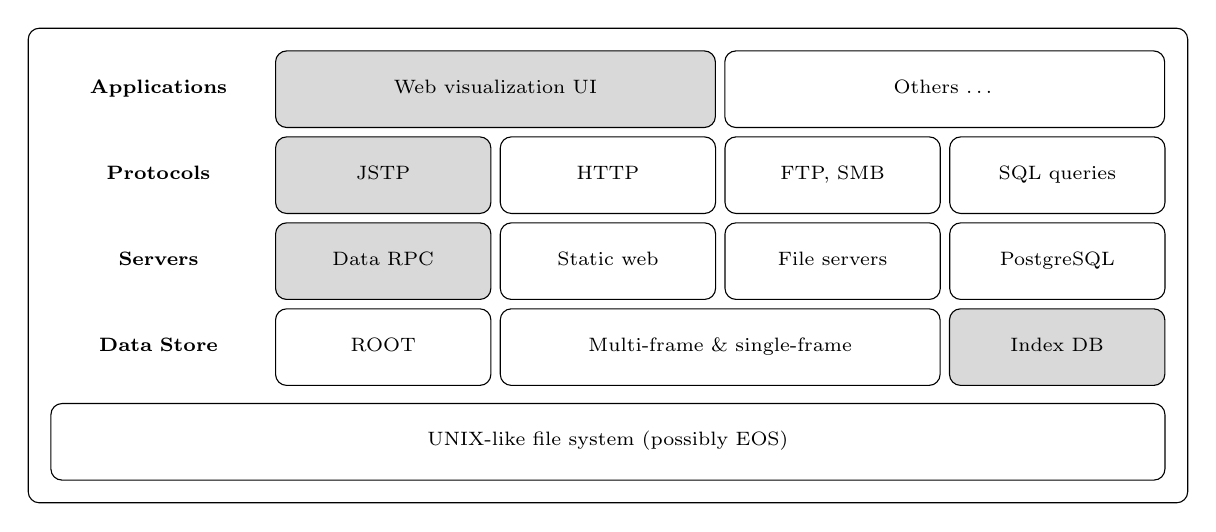
\begin{tikzpicture}[node distance=3pt,
	blueb/.style={
	  draw=black,
	  rounded corners,
	  text width=2.5cm,
	  font=\scriptsize,
	  align=center,
	  text height=12pt,
	  text depth=9pt
	},
	layerb/.style={
	  blueb,
	  draw=none
	},
	proprietaryb/.style={
	  blueb,
	  fill=gray!30
	}]

	\node[layerb] (Clients) {\textbf{Applications}};
	\node[proprietaryb,right=of Clients,text width=5cm+10pt] (VizUI) {Web visualization UI};
	\node[blueb,right=of VizUI,text width=5cm+10pt] (Apps) {Others \dots};

	\node[layerb,below=of Clients] (Protocols) {\textbf{Protocols}};
	\node[proprietaryb,right=of Protocols] (JSTP) {JSTP};
	\node[blueb,right=of JSTP] (HTTP) {HTTP};
	\node[blueb,right=of HTTP] (FileP) {FTP, SMB};
	\node[blueb,right=of FileP] (SQLP) {SQL queries};

	\node[layerb,below=of Protocols] (Servers) {\textbf{Servers}};
	\node[proprietaryb,right=of Servers] (DataS) {Data RPC};
	\node[blueb,right=of DataS] (WebS) {Static web};
	\node[blueb,right=of WebS] (FileS) {File servers};
	\node[blueb,right=of FileS] (SQLS) {PostgreSQL};

	\node[layerb,below=of Servers] (Data) {\textbf{Data Store}};
	\node[blueb,right=of Data] (ROOT) {ROOT};
	\node[blueb,right=of ROOT,text width=5cm+10pt] (MF) {Multi-frame \& single-frame};
	\node[proprietaryb,right=of MF] (SQLD) {Index DB};

	\node[blueb,below=2.4cm of HTTP,text width=13cm+26pt] (FileSystem) {UNIX-like file system (possibly EOS)};

	\begin{pgfonlayer}{background}
	\draw[blueb,draw=black] 
	  ([xshift=-8pt,yshift=8pt]current bounding box.north west) rectangle 
	  ([xshift=8pt,yshift=-8pt]current bounding box.south east);
	\end{pgfonlayer}
	\end{tikzpicture}

\caption{A multi-layered system. Proprietary components are emphasized by gray color.}
\label{fig:multilayered-diagram}
\end{center}
\end{figure}

We may imagine this as follows. Users who want a quick peek at the detector operation without any effort might decide to use the visualization UI in their web browser. The website is quite easy to use, does not require any particular skills to operate, and is capable of displaying frames captured by the detectors as well as overview of their operation. In contrast, users who want to retrieve data for experimentation or statistical aggregation might utilize SQL or JSTP as these two protocols are not designed to interact with humans, but with other applications, most notably utilizable in scripts designed for custom data processing. Lastly, users in need of information, which is not displayed by the visualization UI nor transmitted by any of the mentioned protocols, are welcome to connect to the database storage facility remotely and directly download data files by means of some of the supported network transfer protocols. This concept is illustrated in Figure \ref{fig:multilayered-diagram}.

% CITACE: konkurenční projekty
We should also consider extensibility of JSTP in the future. With multiple concurrent projects such as MoEDAL-TPX\footnote{Similarly to ATLAS-TPX, MoEDAL-TPX is a network of Timepix devices installed within the MoEDAL experiment at CERN.}, SATRAM\footnote{SATRAM is a technology demonstration device carrying Timepix position-sensitive semiconductor pixel detector on board ESA’s Proba V satellite. \url{http://satram.utef.cvut.cz/}} and RISESat\footnote{RISESat is a microsatellite mission carrying several scientific instruments including a Timepix detector.}, it is likely that JSTP will be used for compatibility reasons in other applications as well. It should therefore allow for limited variability, gracefully handling minor alterations in transmitted data structures.

\subsection{Requirements}
Let us now list all formal requirements on JSTP. The most basic one is that the protocol allows us to retrieve frames captured by the ATLAS-TPX network by their start time and device of origin. This might remind us of a similar requirement in the database definition (see section \ref{db:definition}), as it is the most likely user request. However unlike our database, JSTP must be able to transmit only those frames, which satisfy the user predicate, minimizing information overhead in the transmitted messages.

In the first version, we require JSTP only to transmit results of the cluster analysis, leaving door open for pixel matrix transmissions in the future. This indirectly implies that every message transmitted through JSTP containing a captured frame will have to consist of two parts: a header (containing detector configuration, position, orientation, etc.) and a body (containing a list of clusters, or possibly a pixel matrix).

To efficiently reference detectors in the ATLAS-TPX network, we require that JSTP provides an exhaustive list of network elements along with information about their availability in the system. This might seem a bit redundant at first, but consider that JSTP needs to be ready for situations when detectors malfunction, are replaced, or new detectors are installed in the network. These events might not be that uncommon, especially given the experimental nature of the project.

Lastly, in order to aid with navigation in large amounts of detector footage, we require JSTP to offer us a mechanism to generate statistics over larger periods of time. This information will help users find events of interest in overwhelming quantities of white noise, resembling the proverbial \textit{needle in a haystack}.

Apart from various file management network protocols we listed earlier, we do not place any data manipulation requirements on JSTP, implying that the protocol cannot be used for other than read-only access to detector footage.

\section{Underlying Standards}
JSTP is web protocol and as such, it utilizes HTTP as its underlying standard. This allows us to abstract ourselves from caveats of data transmission and compression, and to focus more on the transmitted data instead. By this declaration, we also indirectly  imply that JSTP is a request-response communication protocol between two types of agents: a server and a client. In its architecture, JSTP consists of two parts: a web service providing API for remote procedure calls (RPC) and a data format built atop of it to facilitate these calls. Since JSTP does not include any universal service description mechanism such as WSDL or WADL, all clients need to know its capabilities and calling conventions prior to initiating communication with the server. For data serialization, JSTP utilizes JavaScript Object Notation (JSON). This format has been selected for various reasons. It is simple to parse, offers an extensible tree structure and is very common among web services of this kind, as it is directly supported by the JavaScript client-side runtime used in the web visualization UI. Apart from JSON, JSTP does not offer nor accept communication in any other data formats.

Observant readers may ask whether JSTP web methods meet the standards of RESTful web services. While it is true that the protocol shows many traits often attributed to RESTful services (client-server model, stateless protocol, cacheability, layered system), it certainly does not satisfy all of them. For instance, JSTP does not uniquely identify resources by their URI because it does not offer any of the common CRUD operations. Moreover, in referencing entities, JSTP uses arbitrary identifiers (recall members \texttt{fid}, \texttt{frid} and \texttt{sid} of entities defined in section \ref{db:definition}), which are not passed in the URI but through an array in the request body. Moreover, JSTP does not offer a uniform interface, capable of negotiating data format according to client limitations. Instead, it forces clients to communicate strictly in JSON, adhering to its own data structures and calling conventions.

\section{Web Methods}
\label{jstp:web-methods}
The main component of JSTP is a web service, which can be described as a set of proprietary web methods. For the purpose of simplicity, in this section we provide only a semantical description of each method. Readers interested in full technical documentation of the methods are referred to Appendix \ref{apx:jstp-doc}.

\subsection{Detector List}
The first method is dedicated to providing an updated list of operational detectors in the ATLAS-TPX network.

As we mentioned earlier, we need to be ready for situations when the physical structure of the network changes due to malfunctions or upgrades. For these reasons, any client intending to retrieve frames from a specific detector must first consult the list provided by this method to verify, whether the device is still connected and operational. In addition, other clients unaware of the network's architecture may use this method to obtain an exhaustive listing of all currently available data sources.

Execution of this method requires no parameters. The server responds by transmitting a list of devices, from which data can be retrieved at the time of request. For detailed documentation of this method including examples of requests and responses, see section \ref{apx:jstp-sensors} of the Appendix.

\subsection{Overview of Acquisition}
To satisfy demands on navigation in voluminous amounts of data, we dedicate the second web method to providing an overview on detector acquisition. This is achieved by uniformly dividing a specific time period into finitely many time intervals, in which all relevant frames are gathered with respect to their start time (acquisition time is not considered). In every interval, frames are subsequently processed to produce aggregate statistics, which might indicate time points, where frames of interest are located. This approach is in its essence very similar to the binning procedure used when constructing histograms.

Clients calling this method are required to transmit five parameters in their request:

\begin{description}
	\item[Detector Predicate]
	A group of detector identifiers, restricting all processed frames by their device of origin.

	\item[Start Time, End Time]
	These parameters define the time period, in which we generate statistics. Obviously, the first parameter must be an earlier point of time than the latter.

	\item[Group Period]
	The duration of every interval in the partitioning of the time period. Should an imperfect partitioning occur, the number of intervals is always rounded up to the nearest integer, possibly exceeding the specified end time.

	Longer durations obviously result in a lower number of intervals, and in turn a lower number of returned data points. Shorter durations yield more data points, but may result in lengthy processing at server-side. For stability reasons, the server therefore requires that the duration of the group period results in at least 1 and at most 1024 intervals.

	\item[Normalized Mode]
	An option to compensate possible data distortions caused by variations in frame acquisition times. This setting is irrelevant in configurations, where users can be certain such variations do not occur.
\end{description}

If the server finds request parameters to be valid and succeeds in generating requested statistics, it responds by transmitting a list of data points, corresponding with intervals of the partitioning of the specified time period. Every data point includes three values:

\begin{description}
	\item[Cluster Counts]
	Sums of cluster counts from every frame in the interval, summed separately per every of the six cluster types (for type definitions, see section \ref{db:shape-classification}).

	\item[Frame Occupancy]
	Total number of non-zero pixels in all frames in the interval, indicating their levels of saturation.

	\item[Number of Frames]
	The count of frames aggregated in the interval.
\end{description}

For detailed documentation of this method including examples of requests and responses, see section \ref{apx:jstp-timeline} of the Appendix.

\subsection{Frame Search}
The third method serves to retrieve frames captured at any given point in time by a detector (or a group of detectors). As the method's name might suggest, time need not be exact, resulting in a search for the nearest frame operating on the scope of the index database. There are several search modes available, each offering a different strategy to find \textit{the master frame}. Once such frame is identified, its start time is then used to locate other frames from the remaining detectors, yielding at most one frame per every detector. In the first version of JSTP, we support two search modes:

\begin{description}
	\item[Sequential Forward Mode]
	The master frame is the frame with the start time nearest to, but greater or equal than the time parameter of the search.

	\item[Sequential Backward Mode]
	The master frame is the frame with the start time nearest to, but lower or equal than the time parameter of the search.

	%\item[Sequential Omnidirectional Mode]
	%\item[Exact Match Mode]
\end{description}

Let us demonstrate operation of these modes on a real world example. Suppose that we are interested in frames captured by two devices. Detector 1 captures frames every 0.25 seconds with acquisition time of 0.05 seconds, whereas detector 2 captures frames every 0.33 seconds with acquisition time of 0.27 seconds. If we set the search time to 0.4 seconds and search in the forward mode, the third frame captured by detector 1 will be designated as the master frame. Since the start time of this frame is 0.5 seconds, the second chosen frame will be the second frame captured by detector 2 as its start time is 0.33 seconds and its end time is 0.6 seconds. This scenario is depicted in Figure \ref{fig:frame-search-forward}. If we to use the backward mode instead, the second frame captured by detector 2 will be designated as the master frame. Since its start time is 0.33 seconds and there is a gap in detector 1 footage between 0.3 seconds (end time of the second frame) and 0.5 seconds (start time of the third frame), the algorithm will return no frame for the other detector. This is illustrated in Figure \ref{fig:frame-search-backward}.

% TODO: doplnit dva obrázky

\begin{figure}[t]
\begin{center}
	\begin{subfigure}[b]{0.4\textwidth}
	\Large
	\begin{tikztimingtable}
		\textnormal{D1}   & zz D{1}zzzz D{2}zzzz D{3}zzzz ;[fill=yellow!50]D{4};[fill=none] zzzz D{}         \\
		\textnormal{D2}   & zz 5D{1}z ;[fill=gray!30]5D{2};[fill=none]z 2D{}  \\
		\textnormal{D3}   & zz 2D{1}z   2D{2}z   2D{3}z   ;[fill=gray!30]2D{4};[fill=none] z    2D{5}z 0.5D{}   \\
		\extracode
	\begin{pgfonlayer}{background}
	\vertlines[help  lines]{1,9,10,13}
	\end{pgfonlayer}
	\end{tikztimingtable}
	\caption{Forward search.}
	\label{fig:frame-search-forward}
	\end{subfigure}
	~ %spacing
	\begin{subfigure}[b]{0.4\textwidth}\Large
	\begin{tikztimingtable}
		\textnormal{D1}   & zz D{1}zzzz D{2}zzzz D{3}zzzz D{4}zzzz D{}         \\
		\textnormal{D2}   & zz 5D{1}z ;[fill=gray!30]5D{2};[fill=none]z 2D{}  \\
		\textnormal{D3}   & zz 2D{1}z   2D{2}z   2D{3}z   ;[fill=yellow!50]2D{4};[fill=none] z    2D{5}z 0.5D{}   \\
		\extracode
	\begin{pgfonlayer}{background}
	\vertlines[help  lines]{1,8.5,9,13}
	\end{pgfonlayer}
	\end{tikztimingtable}
	\caption{Backward search.}
	\label{fig:frame-search-backward}
	\end{subfigure}

\caption{Time diagram of frame search illustrating behavioral differences between search modes. Individual blocks correspond with periods of detector acquisition. Emphasized blocks are returned as the search result (yellow marks the master frame).}
\label{fig:frame-search}
\end{center}
\end{figure}

To summarize, clients calling this method are required to specify four parameters:
\begin{description}
	\item[Time of Search]
	The point in time used as a starting point of the search.

	\item[Detector Predicate]
	A group of detector identifiers, restricting retrieved frames by their device of origin.

	\item[Search Mode]
	A strategy to select the master frame based on the time of search and available detector footage.

	\item[Integral Frames]
	Number of consecutive frames to be integrated for every device.
\end{description}

If the server finds request parameters to be valid and succeeds in locating at least one frame, it responds by transmitting the start time of the master frame, followed by headers and bodies of all found frames, corresponding with the order of identifiers in the detector predicate of the request. Frame bodies are transmitted in the form of cluster lists (for properties of clusters, see section \ref{db:cluster-properties}). Detailed documentation of this method, including examples of requests and responses, is available in section \ref{apx:jstp-frame} of the Appendix.

\section{Miscellaneous}
JSTP has been originally designed to serve solely as a data transmission component of the visualization UI. Over time, it has however grown to be a more complex protocol, with applications in other projects than ATLAS-TPX and outside the conventional task of data visualization. It is the intention of author to continue development of this protocol with further releases in the future, eventually decoupling it from the Timepix chip and abstracting it to the point where it could be utilized in combinations with different hardware.

Since the amount of data in our database is expected to become rather overwhelming, the protocol itself is structured and meant to be used in a top-down model (see Figure \ref{fig:jstp-uml}), allowing clients to gradually refine parameters of their requests and locate the information they seek, while avoiding transmission of data in overly granular bulks. In other cases, the protocol minimizes information overhead by requiring strong usage of predicates operating on the index database.

Note that in the protocol definition, we do not specify whether the results of individual web method calls are cacheable by clients. This is due to the diversified nature of its applications. Since HTTP already contains its own caching logic\footnote{Caching in HTTP is controlled by values of headers provided in every response message. Relevant header names are: \texttt{Cache-Control}, \texttt{Expires} and \texttt{Pragma}.}, we encourage all clients to comply with strategies described in \cite{HTTP1999}, section 13, as JSTP servers are permitted to use this mechanism to emply different caching policies for individual response messages. Analogous declaration is used for data compression (for HTTP specification, see section 3.5 of \cite{HTTP1999}).

\begin{figure}[t]
\begin{center}
	\begin{sequencediagram}
		\newthread{c}{:JstpClient}
		\newinst[2]{s}{:JstpServer}
		\newinst[1]{idb}{:IndexDatabase}
		\newinst{fdb}{:FileDatabase}

		\begin{call}{c}{detectorList()}{s}{device list}
			\begin{call}{s}{selectSensors()}{idb}{device list}
			\end{call}
		\end{call}
		
		\begin{sdblock}{Until significant data is found}{}
			\begin{call}{c}{acqOverview()}{s}{statistics}
				\begin{call}{s}{selectFiles()}{idb}{affected files}
				\end{call}
				\begin{call}{s}{selectFrames()}{idb}{statistics}
					\begin{callself}{idb}{\small aggregate()}{}
					\end{callself}
				\end{call}
			\end{call}
		\end{sdblock}
		
		\begin{call}{c}{frameSearch()}{s}{found frames}
			\begin{call}{s}{selectFrames()}{idb}{master frame}
			\end{call}
			\begin{sdblock}{For every device}{}
				\begin{call}{s}{selectFrames()}{idb}{entry indices}
				\end{call}
				\begin{call}{s}{readFile()}{fdb}{frame contents}
				\end{call}
			\end{sdblock}
		\end{call}
	\end{sequencediagram}

\caption{UML diagram depicting expected interactions between JSTP client and server, hinting levels of processing complexity at server-side.}
\label{fig:jstp-uml}
\end{center}
\end{figure}










\chapter{Data Server}
% 4. Datový server
This chapter describes implementation of a JSTP server in C++. While sections in the beginning focus on the role of the server in the entire visualization system and its connection to other components of the application, the sections in the end give details on its operation and propose performance optimizations.

\section{Role of the Application}
%  - Volba povahy serverové aplikace s ohledem na zbylé části systému.
It has been already mentioned in the definition of JSTP that the primary purpose of the protocol is to facilitate connection between the web visualization UI and the ATLAS-TPX footage database. Since the database is located at the server side, the main responsibility of the JSTP server is to decode stored TPX frames from data files and encode them in JSTP messages as efficiently as possible.

To achieve this goal, the server is expected to interact with not only with its underlying file system (which may be replaced by EOS in the future), but also with the index database. Using the index, the server can accelerate time-based queries, as described in section \ref{db:performance-optimization}.

\todo
% DOPLNIT

\section{Decomposition}
%  - Dekompozice úloh serveru do jednotlivých komponent.
The server consists of two major components, an HTTP thread pool and a ROOT transcoder. As the name suggests, the thread pool is responsible mainly for handling outbound HTTP connections, whereas the transcoder ensures fast consumption of data stored in the ROOT file format.

\subsection{HTTP Thread Pool}
The thread pool is a standard component in many other server applications. It allows simultaneous communication with multiple clients, provided that server's hardware offers parallel processing support.

At the startup, multiple \textit{worker threads} are created. These threads are immediately suspended to conserve server's resources. When a new request arrives, one of the suspended threads is awakened and notified to process the request, compose and send a response. During this operation, the thread is said to be \textit{busy} and cannot receive new requests. Should such a request arrive at that time, the server would opt to awaken another of the suspended threads, gradually exhausting its pool. After the response is sent, the thread returns to suspended state, awaiting further instructions. This way, threads are recycled within the pool throughout server operation.

Each worker thread manages its own separate set of resources, allowing it process requests autonomously. Since such processing occupies a single core of server's CPU, it follows that the total number of threads corresponds\footnote{The correspondence need not be exact. For instance, when testing the application on machines with 2, 4 or 8 cores, the most effective number of threads was equal to the number of cores multiplied by 4.} with the number of cores in the CPU.

Apart from reading and writing to the HTTP socket, worker threads are responsible for choosing the correct behavior in order to respond to requests in compliance with the JSTP specification. For instance, every web method listed in section \ref{jstp:web-methods} is represented by a separate \textit{request handler}. Upon request, a worker thread decides which method is being called, creates a corresponding handler, and gives it abstracted control over the HTTP socket. After the handler is finished processing the request, the worker thread sends the response to the client and destroys the handler, freeing up resources related to the communication session.

\subsection{ROOT Transcoder}
The primary purpose of the transcoder is to access detector footage stored within ROOT data files and convert it to JSTP messages. Unlike the thread pool, the transcoder is not a single object but rather a dedicated set of tools and objects designed to efficiently handle large amounts of data.

Recall from section \ref{storage:ROOT} that the ROOT format stores information in tree structures, separating detector configuration from cluster lists. Due to possibly overwhelming sizes of data files, it is nontrivial to devise logic to minimize access time with respect to memory paging and L1 cache. Some of the most significant factors to consider are:

\begin{description}
	\item[ROOT Compression]
	The ROOT data format utilizes its own compression algorithm, roughly equivalent to the ZIP format in its efficiency. There are multiple levels of compression ranging from the best compression ratio to the fastest reading time. Choice of the compression level affects all subsequent processing required to encode and decode data.

	\item[ROOT Cache]
	In sequential reading, the ROOT data format implicitly uses a file cache to prefetch all buffers for the selected data in the memory.

	\item[Tree Switching]
	When retrieving frame data, switching from the \texttt{dscData} tree to the \texttt{clusterFile} tree and back might cause OS to swap memory every time a single frame is read, producing unnecessary overhead and slowing down the process.

	\item[Data Demand]
	In many instances of JSTP messages, it is requested that only a part of the stored data is read. ROOT allows applications to specify this information prior to initiating sequential reading, and in turn accelerate some procedures.
\end{description}

\section{Dependencies}
%  - Volba knihoven a závislostí, požadavky na kompatibilitu s cílovým systémem.

\section{Object-Oriented Design}
%  - Abstrakce technické vrstvy pomocí polymorfismu, další použité návrhové vzory.

\section{A Note on Parallelism}
%  - Poznámka o vícevláknovém provozu serveru.

\section{Performance Optimizations}
%  - Akcelerace výkonu pomocí sjednoceného přístupu k souborům. Dopady této techniky na alokaci paměti.
%  - Analýza efektivity aplikace: výkonový test, rozbor úniků paměti a řešení některých z nich.

\chapter{Conclusion}

\section{Data Import}
Since the JSTP server uses the index database to locate data files based on any given start time, all data files subject to visualization must be stored in the ROOT format and referenced in the \texttt{rootfiles} SQL table.

Accounting for the ever-growing nature of ATLAS-TPX footage, a periodical prodcedure needs to be performed every time new data arrives from CERN, in order to keep the visualization UI up-to-date. At the time of writing this work, this procedure is semi-automated and initiated manually every day by the researchers at IEAP.

\subsection{Processing Stages}
At CERN, the control PC generates raw data files from the read-out interface of every detector in the network. Data is produced on a hourly basis and saved in the form of multi-frame files. Using FTP, these files are transferred into a temporary directory on the target hard drive. When all file transfers are completed and the validity of files is confirmed, several scripts designed to check consistency of detector acquisition are executed. These scripts analyze contents of received files, reading common configuration values such as the acquisition time or bias voltage, and attempt to find variations between individual frames.

Should these scripts succeed in detecting suspicious values, the files in question are moved into a separate directory and await further inspection by researchers. Otherwise, they move on to the next stage of processing. In this stage, captured frames are subjected to the cluster analysis (for more information about this process, see section \ref{intro:cluster-analysis}). Should the frames be captured in the TOT mode, at this point calibration data is used in combination with the method described in \cite{Jakubek2011S262} to calculate energy values. At the end of this process, ROOT files are produced.

Since the original multi-frame files are not needed anymore, they can be discarded without data loss (or compressed for the purposes of long-term archiving). The ROOT files are moved from the temporary directory to their final location on the hard drive containing the ATLAS-TPX footage database. Subsequently, a dedicated instance of the JSTP data server application is configured to generate information in the index database, in effect registering them for retrieval of JSTP information. From this point onward, the JSTP server as well as the web visualization UI are able to read frames stored within newly added files.

\subsection{Automation of the Procedure}
\label{import-automation}
At the present time, the procedure of extending TPX database with new footage is time-consuming as its processing stages often perform similar operations repeatedly for diferent purposes. For example, a single enumeration of multi-frame files should suffice both for consistency checking and cluster analysis. Furthermore, index data corresponding with produced ROOT files can be generated at the time of their production.

It is however worth noting that this procedure was originally designed in the fall of 2015 with the sole purpose of transferring data from CERN to IEAP. Its automation is currently under investigation.

\section{Future of the Application}
At the time of writing this work, the server application is hosted at IEAP. The web visualization UI is publicly accessible online\footnote{\url{http://atlastpx.utef.cvut.cz}}, periodically updated with the latest ATLAS-TPX footage. Its internal components consitute a rudimentary data warehouse, which not only offers several terabytes of research data, but also serves to further promote scientific works done by IEAP, CTU, ATLAS and Medipix collaboration at CERN.

In the future, the physical machine hosting the application is expected to be upgraded and relocated to CERN. Consequently, the JSTP server would be updated for compatibility with EOS, which would be used to substitute a conventional file system. The PostgreSQL server used to manage the index database could be also replaced by CERN's OnDemandDb service. Moreover, while hosted at CERN, the JSTP server may be modified to directly receive data streams of captured information in the multi-frame format and process them automatically in a queue. This setup might reduce the time interval between data acquisition and visualization from days to hours or possibly even minutes, with respect to the limitations of hardware and local area network available at CERN.

A slightly modified version of the server application might also be utilized to offer access to footage captured by TPX detectors installed in different experiments operated in collaboration with IEAP. At the present time, the author of this work is investigating its possible deployment in the MoEDAL experiment CERN and the RISESat satellite collaboration. In the end, it is his belief that this application has the potential to become an data visualization software for any scientific experiment gathering data from TPX detectors, capable of efficiently operating with big amounts of research data.


%%%%%%%%%%%%%%%%%%%%%%%%%% 
% Seznam literatury je v samostatnem souboru reference.bib. Ten
% upravte dle vlastnich potreb, potom zpracujte (a do textu
% zapracujte) pomoci prikazu bibtex a nasledne pdflatex (nebo
% latex). Druhy z nich alespon 2x, aby se poresily odkazy.

% originally following specification for bibliography formating was used
%\bibliographystyle{abbrv}

% Here is an improvment by Petr Dlouhy (April 2010).
% It is mainly for supervisors who expect Czech fomrating rules for references
% Additional feature is live url addresses to sources from your pdf file
% It requires the file csplainnat.bst (included in this sample zipfile).

%\bibliographystyle{csplainnat}

\bibliographystyle{plain}
%\bibliographystyle{psc}
{
%JZ: 11.12.2008 Kdo chce mit v techto ukazkovych odkazech take odkaz na CSTeX:
\def\CS{$\cal C\kern-0.1667em\lower.5ex\hbox{$\cal S$}\kern-0.075em $}
\bibliography{reference}
}

% M. Dušek radi:
%\bibliographystyle{alpha}
% kdy citace ma tvar [AutorRok] (napriklad [Cook97]). Sice to asi neni  podle ceske normy (BTW BibTeX stejne neodpovida ceske norme), ale je to nejprehlednejsi.
% 3.5.2009 JZ polemizuje: BibTeX neobvinujte, napiste a poskytnete nam styl (.bst) splnujici citacni normu CSN/ISO.


%%%%%%%%%%%%%%%%%%%%%%%%%% 
% vše co následuje bude uvedeno v přílohách
\appendix

\chapter{Index Database Scripts}
This appendix contains PostgreSQL scripts used to define the data structure of the index database.

\section{Access Roles}
To access the database, two user roles are created. While the first allows read-only access, the latter also permits users to modify the data.
~
\inputsql{code/security.sql}

\section{Tables}
All index data is stored in the form of SQL table rows. This section contains definition of three tables, capable of persisting information further described in section \ref{db:definition}.

\subsection{Detector Table}
\inputsql{code/sensors.sql}

\subsection{File Table}
\inputsql{code/rootfiles.sql}

\subsection{Frame Table}
\inputsql{code/frames.sql}

\chapter{Documentation of JSTP Web~Methods}
\label{apx:jstp-doc}
This chapter includes detailed documentation of the JSTP web service along with protocol conventions, parameter descriptions and examples of requests and responses.

\section{API Conventions}
\begin{enumerate}
	\item
	When referring to the HTTP endpoint of the web service in method URLs, ``\texttt{<endpoint>}'' is used as a stand-in string.

	\item
	All date and time information is transmitted as the number of seconds from the midnight of January 1, 1970 (in UTC). Durations are transmitted in seconds and energies in keV.

	\item 
	JSTP responses support HTTP status codes: 200 (OK), 400 (Bad Request), 404 (Not Found) and 500 (Internal Server Error).

	\item
	All JSTP web methods use the JSON format for serialization of request parameters and response data. When parameters are required, the server expects the client to initiate a POST request, passing their values in a JSON object as a part of the post data. Unless specified otherwise, all method parameters are mandatory.
\end{enumerate}

\section{Detector List}
\label{apx:jstp-sensors}
To execute this method, a client must initiate a GET request to \texttt{<endpoint>/sensors} without any parameters. When successful, the server responds by returning an array of objects, each of which corresponds to a single device in the TPX network. Example of such response is provided in Listing \ref{lst:jstp-sensors}. Every object in the array is guaranteed to contain:
~
\begin{description}
	\item[\texttt{sid}]
	Unique numeric identifier of the device retrieved from the index database.

	\item[\texttt{name}]
	Readable name of the device.
\end{description}

\begin{listing}
	\inputjson{code/jstp-sensors.json}
    \caption[JSTP detector list response body.]{Example response containing a list of two devices.}
    \label{lst:jstp-sensors}
\end{listing}


\section{Overview of Acquisition}
\label{apx:jstp-timeline}
To execute this method, a client must initiate a POST request to \texttt{<endpoint>/timeline}. The request body must contain a JSON object with \textit{all} parameter values. You can examine an example request body in Listing \ref{lst:jstp-timeline-request}.

\begin{listing}
	\inputjson{code/jstp-timeline-request.json}
    \caption[JSTP acquisition overview request body.]{Example request body with time period starting at July 28, 2015 at 3:00 AM and ending at 6:00 AM. Data from 2 detectors is requested to be normalized and grouped by every hour. Response is expected to contain exactly 3 intervals.}
    \label{lst:jstp-timeline-request}
\end{listing}

When successful, the server responds by returning an array of objects, each of which responds to a single interval in the time period. For example response, see Listing \ref{lst:jstp-timeline-response}. Every object in the array is guaranteed to contain:
~
\begin{description}
	\item[\texttt{time}]
	Start time of the interval. End time of the interval can be calculated at by adding \texttt{groupPeriod} to this value.

	\item[\texttt{frames}]
	Number of frames aggregated in the time interval.
	
	\item[\texttt{occupancy}]
	Count of non-zero pixels in all aggregated frames, indicating the levels of saturation. The maximum possible occupancy is equal to the product of pixels in a single sensor layers, the number of sensor layers and the number of aggregated frames in the interval.
	
	\item[\texttt{counts}]
	Array of counts of clusters in all aggregated frames, differentiated by their type classification. Counts are provided in the order: dots, small blobs, heavy blobs, heavy tracks, straight tracks, curly tracks.

	If the calculations are normalized, individual contributions to these counts from every frame are divided by frame's acquisition time, yielding overall flux instead of counts.
\end{description}

\begin{listing}
	\inputjson{code/jstp-timeline-response.json}
    \caption[JSTP acquisition overview response body.]{Example response to the request from Listing \ref{lst:jstp-timeline-request}.}
    \label{lst:jstp-timeline-response}
\end{listing}

\section{Frame Search}
\label{apx:jstp-frame}
To execute this method, a client must initiate a POST request to \texttt{<endpoint>/frame}. The request body must contain a JSON object with \textit{all} parameter values:
~
\begin{description}
	\item[\texttt{time}]
	The search time parameter.

	\item[\texttt{sensors}]
	Array of distinct \texttt{sid} values of the devices, from which we wish to retrieve data. This array must not be empty.

	\item[\texttt{searchMode}]
	A non-negative integer value specifying the algorithm to be used in the search operation. Possible values are 0 (Sequential Forward Mode) and 1 ( Sequential Backward Mode).

	\item[\texttt{integralFrames}]
	A positive integer not greater than 100 controlling the number of frames integrated in time. Value equal to 1 retrieves only a single frame. This value must be equal to 1 when frames from more than one device are requested.
\end{description}

\begin{listing}
	\inputjson{code/jstp-frames-request.json} % TODO
    \caption[JSTP frame search request body.]{Example request body with time parameter equal to July 28, 2015, 3:00 AM. A single frame captured by a single detector is requested to be located by the Sequential Forward Mode.}
    \label{lst:jstp-frames-request}
\end{listing}

For an example request, see Listing \ref{lst:jstp-frames-request}. In response, the server returns an object containing \texttt{foundTime}, the start time of the master frame, and \texttt{frames}, an array of objects corresponding with frames captured by every device in the order, in which they were referenced in the \texttt{sensors} array. Every object is guaranteed to contain:
~
\begin{description}
	\item[\texttt{rootFile}]
	Path to the ROOT file, from which this frame was extracted (in the server's file system).

	\item[\texttt{rootFrameIndex}]
	Index of the entry in ROOT file's \texttt{dscData} tree, containing information about detector configuration.

	\item[\texttt{rootFirstClusterIndex}]
	Index of the first entry in ROOT file's \texttt{clusterFile} tree, corresponding with the first cluster in the frame. If no such entry exists, this value is null or negative.

	\item[\texttt{layers}]
	Number of detector's sensor layers.

	\item[\texttt{startTime}]
	The start time of acquisition.

	\item[\texttt{acquisitionTime}]
	The acquisition time (the length of acquisition) in seconds.

	\item[\texttt{biasVoltage}]
	The array of bias voltages of the active sensor layers of the TPX detector.

	\item[\texttt{mode}]
	Operation mode of the TPX detector. Possible values are: MPX (0), TOT (1), one-hit (2), TOA (3), mixed (4). For more information, see Section \ref{section:operation-modes}.

	\item[\texttt{chipboardId}]
	The identifier of the hardware used in the TPX detector.

	\item[\texttt{maskedPixels}]
	The number of masked pixels at the time of acquisition.

	\item[\texttt{layerNames}]
	The array of human-readable labels for the active sensor layers of the TPX detector.

	\item[\texttt{calibrationConstants}]
	The array of constants, which can be used in conjunction with TOT data to calculate instantaneous luminosity estimation for every active sensor layer. These constants are available only for some devices.

	\item[\texttt{position}]
	Position of the TPX detector within the ATLAS machine's coordinate system.

	\item[\texttt{clusters}]
	Sparse array of clusters found in the frame. Each cluster is represented by a separate JSON object. The ordering of such objects is not defined.
\end{description}

Every object in the \texttt{clusters} array is guaranteed to contain:
~
\begin{description}
	\item[\texttt{x}]
	Array of X coordinates of the pixels in the cluster.

	\item[\texttt{y}]
	Array of Y coordinates of the pixels in the cluster.

	\item[\texttt{counter}]
	Array of counter values of the pixels in the cluster.

	\item[\texttt{energy}]
	Array of energy values of the pixels in the cluster (available only in the TOT mode).

	\item[\texttt{entry}]
	Index of the entry in ROOT file's \texttt{clusterFile} tree, corresponding to this cluster.

	\item[\texttt{layer}]
	Number of the active sensor layer, to which the cluster belongs.

	\item[\texttt{type}]
	Nonnegative integer determining the type classification of the cluster. Possible values are: dot (1), small blob (2), heavy blob (3), heavy track (4), straight track (5) and curly track (6). For more information, see Figure \ref{fig:cluster-types}.

	\item[\texttt{size}]
	The number of pixels in the cluster.

	\item[\texttt{roundness}]
	Morphological value describing the roundness of the cluster.

	\item[\texttt{linearity}]
	Morphological value describing the linearity of the cluster.

	\item[\texttt{region}]
	Nonnegative integer determining the region of the active sensor layer, in which the cluster is located. Possible values are: mixed (0), silicon (1), polyethylene (2), polyethylene with aluminum (3), lithium fluoride (4).

	\item[\texttt{energyMaxHeight}]
	The highest energy value of the pixels in the cluster (available only in the TOT mode).

	\item[\texttt{energyMinHeight}]
	The lowest energy value of the pixels in the cluster (available only in the TOT mode).

	\item[\texttt{energyVolume}]	
	The sum of energy values of the pixels in the cluster (available only in the TOT mode).

	\item[\texttt{counterMaxHeight}]
	The highest counter value of the pixels in the cluster.

	\item[\texttt{counterMinHeight}]
	The lowest counter value of the pixels in the cluster.

	\item[\texttt{meanX}]
	The average X coordinate of the pixels in the cluster.

	\item[\texttt{meanY}]
	The average Y coordinate of the pixels in the cluster.

	\item[\texttt{volCentroidX}]
	The average X coordinate of the pixels in the cluster, weighted by counter values.

	\item[\texttt{volCentroidY}]
	The average Y coordinate of the pixels in the cluster, weighted by counter values.
\end{description}


\printnomenclature
\label{apx:zkratky}

\chapter{Contents of the Attached DVD}
\begin{figure}[h]
\begin{center}

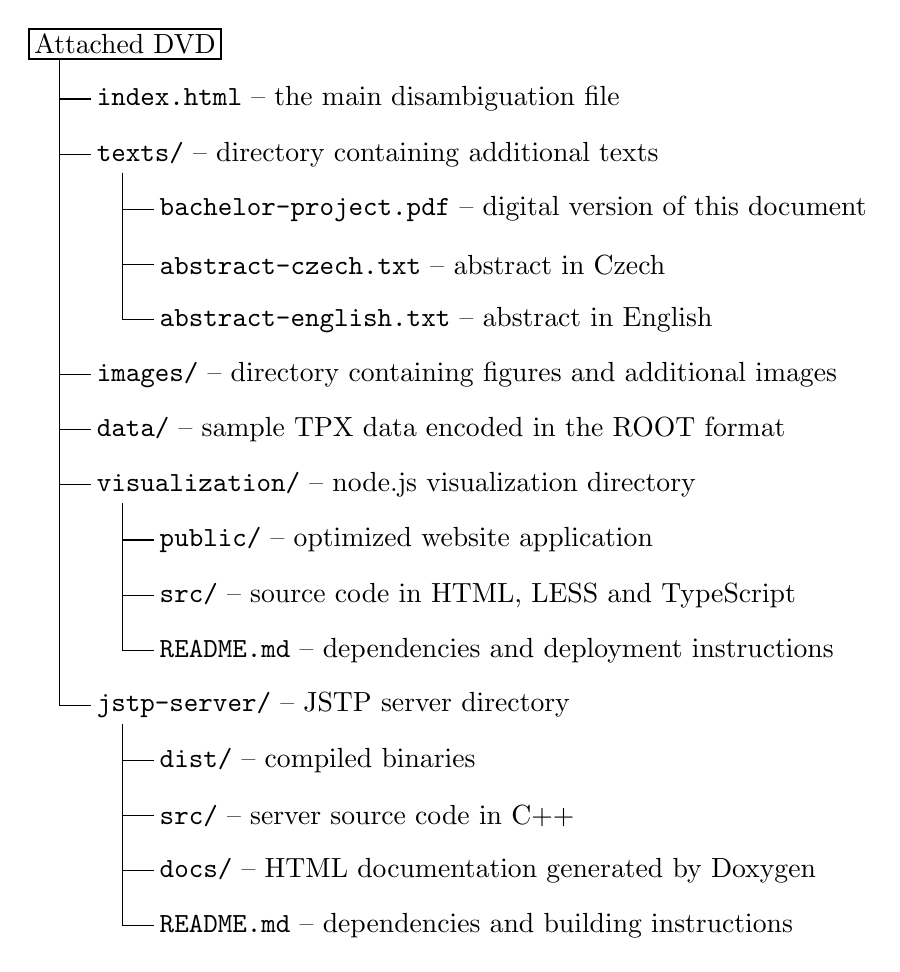
\begin{tikzpicture}[
    every node/.style={
        anchor=west,
        inner sep=2pt,
        minimum size=1pt,
    },
    grow via three points={
        one child at (0.8,-0.7) and two children at (0.8,-0.7) and (0.8,-1.4)
    },
    edge from parent path={
        ($(\tikzparentnode\tikzparentanchor)+(.4cm,0pt)$) |- (\tikzchildnode\tikzchildanchor)
    },
    growth parent anchor=west,
    parent anchor=south west
  ]
  \node [draw=black,thick] {Attached DVD}
    child { node {\texttt{index.html} -- the main disambiguation file}}
    child { node {\texttt{texts/} -- directory containing additional texts} 
    	child { node {\texttt{bachelor-project.pdf} -- digital version of this document}}
    	child { node {\texttt{abstract-czech.txt} -- abstract in Czech}}
    	child { node {\texttt{abstract-english.txt} -- abstract in English}}
    }
    child [missing] {}
    child [missing] {}
    child [missing] {}
    child { node {\texttt{images/} -- directory containing figures and additional images}}
    child { node {\texttt{data/} -- sample TPX data encoded in the ROOT format}}
    child { node {\texttt{visualization/} -- node.js visualization directory}
    	child { node {\texttt{public/} -- optimized website application}}
    	child { node {\texttt{src/} -- source code in HTML, LESS and TypeScript}}
    	child { node {\texttt{README.md} -- dependencies and deployment instructions}}
    }
    child [missing] {}
    child [missing] {}
    child [missing] {}
    child { node {\texttt{jstp-server/} -- JSTP server directory}
    	child { node {\texttt{dist/} -- compiled binaries}}
    	child { node {\texttt{src/} -- server source code in C++}}
    	child { node {\texttt{docs/} -- HTML documentation generated by Doxygen}}
    	child { node {\texttt{README.md} -- dependencies and building instructions}}
    }    
    child [missing] {}
    child [missing] {}
    child [missing] {}
    child [missing] {};
\end{tikzpicture}

\caption{Contents of the attached DVD}
\label{fig:attached-cd}
\end{center}
\end{figure}

\end{document}
